\begin{figure}[H]
        \subfigure[Tiempo de LOW a HIGH]{
            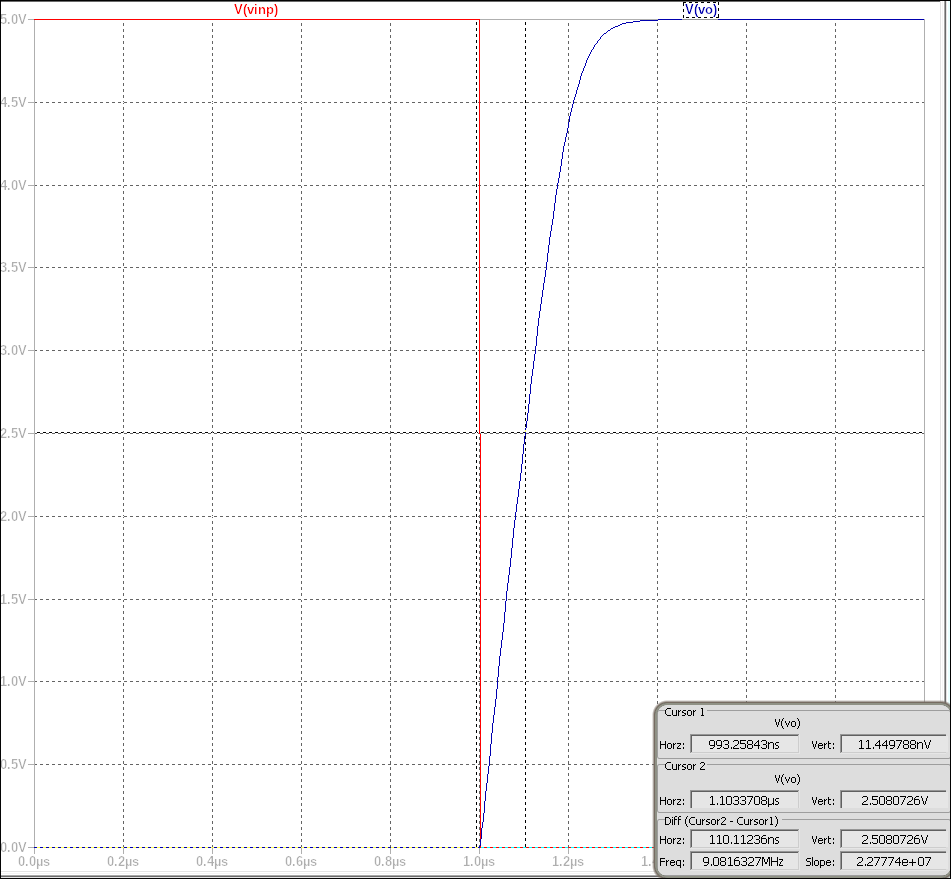
\includegraphics[width=.48\linewidth]{Imagenes/tL2H.png}
            \label{subfig:tL2H}
        }\hfill
        \subfigure[Tiempo de HIGH a LOW]{
            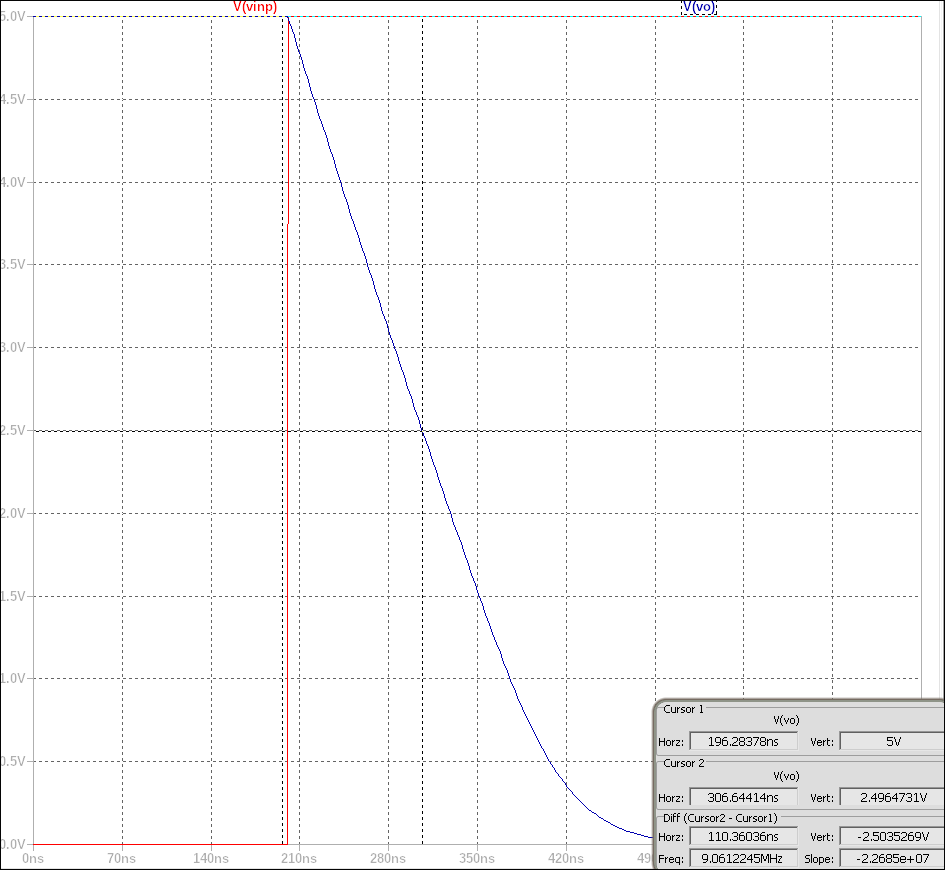
\includegraphics[width=.48\linewidth]{Imagenes/tH2L.png}
            \label{subfig:tH2L}
        }
        \caption{Tiempos de propagación para la compuerta NOT}
        \label{fig: tiempos_propagacion}
\end{figure}

Se puede observar que el tiempo de propagación de HIGH a LOW es de 110.36ns, similar al tiempo de LOW a HIGH que es de 110.1ns.

